\section{Theory}

\subsection{Mathematical Foundation}

Understanding the numerical solution of the heat equation requires familiarity with several key mathematical concepts.
This section introduces the essential notation and theoretical tools we'll use throughout our analysis.

\subsubsection{Notation and Terminology}
The following notation will be used consistently throughout this report:

\begin{table}[h]
  \centering
  \begin{tabular}{@{}ll@{}}
    \textbf{Symbol}          & \textbf{Description}                  \\
    \hline
    $u(x,t)$                 & Temperature at position $x$, time $t$ \\
    $\mu$                    & Diffusion coefficient                 \\
    $f(u)$                   & Reaction term                         \\
    $\Omega, \partial\Omega$ & Domain and boundary                   \\
    \hline
    $h=L/M$, $k=T/N$         & Spatial/temporal step sizes           \\
    $x_m=mh$, $t_n=nk$       & Grid coordinates                      \\
    $u_m^n=u(x_m,t_n)$       & Exact solution at grid point          \\
    $U_m^n$                  & Numerical approximation               \\
    $M$, $N$                 & Number of spatial/temporal points     \\
    $\mathbb{G}$             & Set of all grid points                \\
  \end{tabular}
\end{table}

\subsubsection{Error Analysis Concepts}

A fundamental concept in numerical methods is the local truncation error (LTE), which measures the accuracy of our numerical approximation at each step:

\begin{definition}{Local Truncation Error}{lte}
  The local truncation error quantifies how well a difference equation approximates the exact differential equation at a single step. For a numerical method of order $(p,q)$:
  \[
    \|\tau_m^n\| = \|U_m^n-u(x_m, t_n)\| = \mathcal{O}(h^p + k^q) \quad \text{as} \quad h, k \to 0
  \]
  where $p$ represents the spatial accuracy and $q$ represents the temporal accuracy.
\end{definition}

\begin{definition}{Global Error}{global_error}
  The global error measures the accumulated difference between the numerical solution and the exact solution at a given point:
  \[
    e_m^n = U_m^n - u(x_m, t_n)
  \]
  Unlike local truncation error, global error accounts for the propagation of errors from previous steps.
\end{definition}

\begin{theorem}{Lax Equivalence Theorem}{lax}
  A numerical scheme is convergent if it is both consistent and stable.
  \[
    \operatorname{Consistent} \land \operatorname{Stable} \implies \operatorname{Convergent}
  \]
\end{theorem}

\begin{definition}{Consistency}{consistency}
  A numerical scheme is consistent with a PDE if the local truncation error tends to zero as the step sizes approach zero:
  \[
    \lim_{h,k \to 0} \|\tau_m^n\| = 0
  \]
  A scheme with local truncation error $\mathcal{O}(h^p + k^q)$ is said to be consistent of order $(p,q)$.
\end{definition}

\begin{definition}{Stability}{stability}
  A numerical scheme is stable if small perturbations in the initial data produce bounded changes in the numerical solution. For linear problems, this typically requires the amplification factor $\xi$ to satisfy:
  \[
    |\xi| \leq 1 + Ck
  \]
  for some constant $C$ independent of step sizes.
\end{definition}

\begin{definition}{Convergence}{convergence}
  A numerical scheme is convergent if the global error tends to zero as the step sizes approach zero:
  \[
    \lim_{h,k \to 0} \|e_m^n\| = 0
  \]
  A scheme with global error $\mathcal{O}(h^p + k^q)$ is said to be convergent of order $(p,q)$.
\end{definition}



\subsection{Taylor Series Expansions}\label{sec:taylor_expansions}

Taylor expansions form the backbone of finite difference approximations by allowing us to represent continuous derivatives as discrete differences. When we approximate a derivative using grid points, the accuracy depends on how many terms we retain in the expansion.

\paragraph{Spatial Expansions}
For points neighboring $x_m$:
\begin{align}
  u(x_m + h, t_n) & = u_m^n + h \partial_x u_m^n + \frac{h^2}{2} \partial_x^2 u_m^n + \frac{h^3}{6} \partial_x^3 u_m^n + \mathcal{O}(h^4) \tag{T1} \label{eq:taylor_forward}  \\
  u(x_m - h, t_n) & = u_m^n - h \partial_x u_m^n + \frac{h^2}{2} \partial_x^2 u_m^n - \frac{h^3}{6} \partial_x^3 u_m^n + \mathcal{O}(h^4) \tag{T2} \label{eq:taylor_backward}
\end{align}

\paragraph{Temporal Expansions}
For advancing in time:
\begin{align}
  u(x_m, t_n + k) & = u_m^n + k \partial_t u_m^n + \frac{k^2}{2} \partial_t^2 u_m^n + \frac{k^3}{6} \partial_t^3 u_m^n + \mathcal{O}(k^4) \tag{T3} \label{eq:taylor_time} \\
  u_m^\star       & = u_m^n + \Phi k \partial_t u_m^n + \frac{(\Phi k)^2}{2} \partial_t^2 u_m^n + \mathcal{O}(k^3) \tag{T4} \label{eq:taylor_intermediate}
\end{align}
where $u_m^\star$ represents an intermediate value for a time step $\Phi$ between $t_n$ and $t_{n+1}$.

\paragraph{Mixed Space-Time Expansions}
For points in both space and time:
\begin{align}
  u(x_m + h, t_n + \Phi k) & = u_m^n + h \partial_x u_m^n + \Phi k \partial_t u_m^n + \frac{h^2}{2}\partial_x^2 u_m^n + \mathcal{O}(h^3 + k^2) \tag{T5} \label{eq:taylor_mixed_forward}  \\
  u(x_m - h, t_n + \Phi k) & = u_m^n - h \partial_x u_m^n + \Phi k \partial_t u_m^n + \frac{h^2}{2}\partial_x^2 u_m^n + \mathcal{O}(h^3 + k^2) \tag{T6} \label{eq:taylor_mixed_backward}
\end{align}

\paragraph{Second-Order Central Difference Approximations}
From these expansions, we derive central difference approximations:
\begin{align}
  \delta_x^2 u_m^n     & = u_{m+1}^n - 2u_m^n + u_{m-1}^n = h^2\partial_{xx}u_m^n + \mathcal{O}(h^4) \tag{T7} \label{eq:central_diff}                        \\
  \delta_x^2 u_m^\star & = u_{m+1}^\star - 2u_m^\star + u_{m-1}^\star = h^2\partial_{xx}u_m^n + \mathcal{O}(h^4 + k^2) \tag{T8} \label{eq:central_diff_star}
\end{align}

These approximations makes it possible to construct numerical schemes for solving PDEs.

\subsection{The Heat Equation}

The heat equation is a fundamental partial differential equation (PDE) that governs how temperature evolves in a given region over time. In its simplest form, we consider a one-dimensional case in which heat flows along a single spatial dimension:
\begin{align*}
  \frac{\partial u}{\partial t} & = \mu \frac{\partial^2 u}{\partial x^2} + f(u), \quad \left( x, t \right) \in \Omega \times \left(0, T\right) \tag{PDE} \\
                                &
  \begin{cases}
    u(x, 0) = u_0(x)  &                       \\
    u(0, t) = g(x, t) & x \in \partial \Omega \\
  \end{cases} \tag{BC}
\end{align*}\label{eq:heat_eq}

The equation describes how the temperature \(u(x, t)\) at position \(x\) and time \(t\) evolves over time.

\paragraph{Diffusion and Reaction Terms}
The diffusion term \(\mu \frac{\partial^2 u}{\partial x^2}\) describes how heat spreads through the material, while the reaction term \(f(u)\) accounts for any heat sources or sinks in the system.

\paragraph{Initial and Boundary Conditions}
The initial temperature distribution \(u_0(x)\) and boundary condition \(g(x, t)\) specify the temperature at the start and where heat enters or leaves the system, respectively.

\paragraph{Parabolic PDE}
The heat equation is a \emph{parabolic} PDE describing how processes evolve over time. For numerical solutions, the spatial and temporal domains are discretized, and the solution is approximated at discrete points. Finite difference methods efficiently handle these discretizations, allowing accurate approximations of the evolving temperature.

\subsubsection{Discretization of the Heat Equation}
Discretizing the heat equation involves dividing the spatial domain \(\Omega\) into \(M\) equally spaced points, with \emph{step length \(h\)} and the temporal domain into \(N\) steps, with \emph{step size \(k\)}.
Each grid point is denoted by \((x_m, t_n)\), where \(x_m = m h\) and \(t_n = n k\) for \(m = 0, \ldots, M\) and \(n = 0, \ldots, N\). The solution \(U_m^n\) approximates the temperature \(u(x_m, t_n)\) at each grid point.

\begin{align*}
  U_m^n      & \approx u(x_m, t_n) \quad \text{for } (x_m, t_n) \in \mathbb{G} \\[1em]
  \mathbb{G} & := \left\{(x_m, t_n) \,:\,
  \begin{array}{l}
    x_m = m h, \quad m = 0, 1, \ldots, M \\
    t_n = n k, \quad n = 0, 1, \ldots, N
  \end{array}
  \right\}
\end{align*}\label{eq:grid_points}

Here, $L$ represents the spatial domain length $[0,L]$ and $T$ is the final simulation time.

\begin{remark}{Uniform Grid}{step_sizes}
  For computational simplicity, we use constant step sizes:
  \begin{align*}
    h & = \frac{L}{M} \quad \text{(spatial step size)}  \\
    k & = \frac{T}{N} \quad \text{(temporal step size)}
  \end{align*}
  giving uniform increments: $x_{m+1} = x_m + h$ and $t_{n+1} = t_n + k$.
\end{remark}

\subsection{Finite Difference Schemes}
Finite difference methods approximate differential equations by replacing them with a system of algebraic equations on the chosen grid.
The heat equation is often solved with these methods for their simplicity and computational efficiency.

\paragraph{The Forward-Time Central-Space (FTCS) scheme}
FTSC is a simple and widely used method for solving the heat equation.
It approximates the time derivative with a forward difference and the spatial derivative with a central difference.

\begin{align*}
  \frac{1}{k} \nabla_t U_m^{n+1} & = \frac{\mu}{h^2} \delta_x^2 U_m^{n+1} + f(U_m^n)                                              \\
  \nabla_t U_m^{n+1}             & = r \delta_x^2 U_m^{n+1} + k f(U_m^n), \quad r = \frac{\mu k}{h^2}                             \\
  U_m^{n+1}                      & = U_m^n + r \left( U_{m+1}^{n+1} - 2 U_m^{n+1} + U_{m-1}^{n+1} \right) + k f(U_m^n) \tag{FTCS}
\end{align*}

\paragraph{Crank-Nicolson Scheme}

The Crank-Nicolson scheme is an implicit method that approximates the spatial derivative at the midpoint between time steps. It is unconditionally stable and second-order accurate in time and space.
\begin{align*}
  U_m^\star & = U_m^n + \frac{r}{2} \left( \delta_x^2 U_m^\star + \delta_x^2 U_m^n \right) + k f(U_m^n), \quad r = \frac{\mu k}{h^2} \tag{Crank-Nicolson} \\
  U_m^{n+1} & = U_m^\star + \frac{k}{2} \left( f(U_m^\star) - f(U_m^n) \right)
\end{align*}


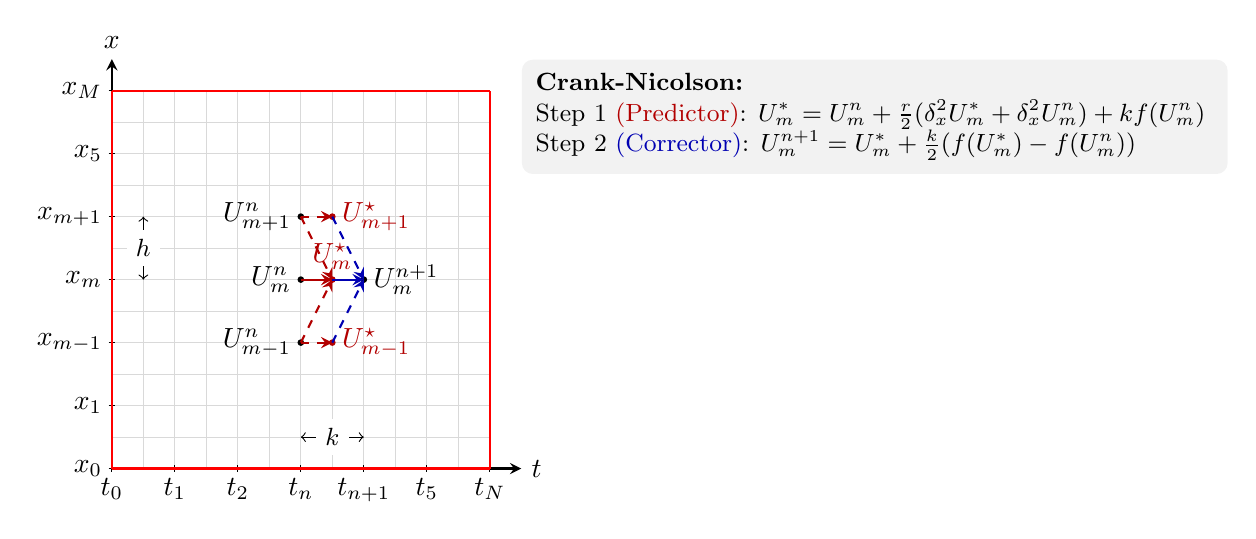
\begin{tikzpicture}[scale=0.8]
  % Define colors
  \colorlet{pointcolor}{black}
  \colorlet{gridcolor}{gray!30}
  \colorlet{predictorcolor}{red!70!black}
  \colorlet{correctorcolor}{blue!70!black}
  
  % Axes
  \draw[-stealth, thick] (0,0) -- (6.5,0) node[right] {$t$};
  \draw[-stealth, thick] (0,0) -- (0,6.5) node[above] {$x$};

  % Grid
    \draw[step=0.5cm, gridcolor, thin] (0,0) grid (6,6);

    % Add time labels
    \foreach \x/\label in {0/0, 1/1, 2/2, 3/n, 4/{n+1}, 5/5, 6/N} {
      \node[below] at (\x,0) {$t_{\label}$};
      \draw (\x,-0.05) -- (\x,0.05);
    }
    
    % Add space labels
    \foreach \y/\label in {0/0, 1/1, 2/{m-1}, 3/m, 4/{m+1}, 5/5, 6/M} {
      \node[left] at (0,\y) {$x_{\label}$};
      \draw (-0.05,\y) -- (0.05,\y);
    }

  % Highlight grid points for Crank-Nicolson stencil
  \fill[pointcolor] (3,3) circle (1.5pt) node[left] {$U_m^n$};
  \fill[pointcolor] (4,3) circle (1.5pt) node[right] {$U_m^{n+1}$};
  \fill[pointcolor] (3,2) circle (1.5pt) node[left] {$U_{m-1}^n$};
  \fill[pointcolor] (3,4) circle (1.5pt) node[left] {$U_{m+1}^n$};
  
  % Add intermediate points for the predictor step
  \fill[predictorcolor] (3.5,3) circle (1.5pt) node[above] {$U_m^\star$};
  \fill[predictorcolor] (3.5,2) circle (1.5pt) node[right] {$U_{m-1}^\star$};
  \fill[predictorcolor] (3.5,4) circle (1.5pt) node[right] {$U_{m+1}^\star$};
  
  % Show the predictor step with arrows
  \draw[->,-stealth, predictorcolor, thick] (3,3) -- (3.5,3);
  \draw[->,-stealth, predictorcolor, thick, dashed] (3,2) -- (3.5,3);
  \draw[->,-stealth, predictorcolor, thick, dashed] (3,4) -- (3.5,3);
  \draw[->,-stealth, predictorcolor, thick, dashed] (3,2) -- (3.5,2);
  \draw[->,-stealth, predictorcolor, thick, dashed] (3,4) -- (3.5,4);
  
  % Show the corrector step with arrows
  \draw[->,-stealth, correctorcolor, thick] (3.5,3) -- (4,3);
  \draw[->,-stealth, correctorcolor, thick, dashed] (3.5,2) -- (4,3);
  \draw[->,-stealth, correctorcolor, thick, dashed] (3.5,4) -- (4,3);
  
  % Step size annotations
  \draw[<->] (3,0.5) -- (4,0.5) node[midway, fill=white, font=\small] {$k$};
  \draw[<->] (0.5,3) -- (0.5,4) node[midway, fill=white, font=\small] {$h$};
  
  % Boundary and initial conditions
  \draw[red, thick] (0,0) -- (0,6);
  \draw[red, thick] (6,0) -- (6,6); 
  \draw[red, thick] (0,0) -- (6,0); 
  \draw[red, thick] (0,6) -- (6,6);
  
  % boundary labels MÅ FIKSES!

  % Crank-Nicolson scheme visualization
  \node[below right, align=left, font=\small, fill=gray!10, rounded corners, inner sep=5pt]
    at (6.5,6.5) {
    \textbf{Crank-Nicolson:}\\
    Step 1 \textcolor{predictorcolor}{(Predictor)}: $U_m^* = U_m^n + \frac{r}{2}(\delta_x^2 U_m^* + \delta_x^2 U_m^n) + k f(U_m^n)$ \hspace{5pt} \\
    Step 2 \textcolor{correctorcolor}{(Corrector)}: $U_m^{n+1} = U_m^* + \frac{k}{2}(f(U_m^*) - f(U_m^n))$
  };
\end{tikzpicture}

\subsection{Error Analysis}
Given the function \(f(u) = au\) for constant \(a\), we first want to analyze the consistency of the Crank-Nicolson scheme by determining the local truncation error (LTE).

\subsubsection{Consistency}
To determine the consistency of the Crank-Nicolson scheme for the heat equation with linear reaction term $f(u) = au$, we analyze the local truncation error by substituting the exact solution into our numerical scheme.

\begin{theorem}{Local truncation error for Crank--Nicolson}{lte_cn}
  For the heat equation $u_t = \mu u_{xx} + au$ with constant $a$, the Crank--Nicolson scheme with steps $h$ (space) and $k$ (time) has local truncation error
  \[
    \|\tau_m^n\| = \mathcal{O}\!\left(k +\tfrac{h^4}{k}\right)
  \]
  where $u_m^n = u(x_m,t_n)$ is the exact solution and $U_m^n$ its numerical approximation.

  Under parabolic scaling $k \sim h^2$, the scheme achieves second-order accuracy:
  \[
    \|\tau_m^n\| = \mathcal{O}\!\left(h^2 + k^2\right)
  \]
\end{theorem}

\begin{proof}[Proof of Theorem~\ref{thm:lte_cn}]
  We analyze the truncation error by examining how the exact solution satisfies the numerical scheme.

  First, consider the central difference approximations for the second derivatives:
  \begin{align*}
    \delta_x^2 u_m^n     & = h^2u_{xx}(x_m,t_n) + \mathcal{O}(h^4)       \\
    \delta_x^2 u_m^\star & = h^2u_{xx}(x_m,t_n) + \mathcal{O}(h^4 + k^4)
  \end{align*}

  \textit{Step 1 (Predictor):} Substituting the exact solution into the first stage:
  \begin{equation}
    u_m^\star = u_m^n + \frac{r}{2}\left(\delta_x^2 u_m^\star + \delta_x^2 u_m^n\right) + kau_m^n = u_m^n + \frac{\mu k}{2}u_{xx}(x_m,t_n) + kau_m^n + \mathcal{O}(h^4 + k^4)
  \end{equation}
  \textit{Step 2 (Corrector):} For the second stage:
  \begin{align*}
    u_m^{n+1} & = u_m^\star + \frac{k}{2}(au_m^\star - au_m^n)
  \end{align*}

  From the PDE, we know $u_t = \mu u_{xx} + au$ and can derive expressions for higher time derivatives. Using Taylor expansion:
  \begin{align*}
    u(x_m,t_n+k) & = u_m^n + ku_t + \frac{k^2}{2}u_{tt} + \frac{k^3}{6}u_{ttt} + \mathcal{O}(k^4)
  \end{align*}

  Comparing this with our numerical solution, we obtain:
  \begin{align*}
    U_m^{n+1} - u_m^{n+1} & = \mathcal{O}(k^2 + h^4)
  \end{align*}

  The local truncation error per step is thus:
  \begin{align*}
    \|\tau_m^{n+1}\| & = \frac{|U_m^{n+1} - u_m^{n+1}|}{k} = \mathcal{O}\left(k + \frac{h^4}{k}\right)
  \end{align*}

  Under the parabolic scaling $k \sim h^2$, we have $\frac{h^4}{k} \sim h^2$, yielding second-order accuracy:
  \begin{align*}
    \|\tau_m^{n+1}\| = \mathcal{O}(h^2 + k^2)
  \end{align*}
\end{proof}

\subsubsection{Stability (Von Neumann)}
\begin{theorem}{von Neumann Stability for Crank--Nicolson}{von_neumann_cn}
  The Crank--Nicolson scheme for the heat equation with linear reaction term $f(u) = au$ is unconditionally stable for any choice of step sizes $h$ and $k$. The amplification factor $\xi$ satisfies:
  \[
    |\xi| \leq 1 + Ck
  \]
  for some constant $C$ independent of step sizes.
\end{theorem}

\begin{proof}[Proof of Theorem~\ref{thm:von_neumann_cn}]
  We apply von Neumann stability analysis by studying how individual Fourier modes $U_m^n = \xi^n e^{i\beta mh}$ evolve under our scheme, where $\beta$ is the wave number.
  
  For the heat equation with linear reaction term $f(u) = au$, the two-stage Crank--Nicolson scheme is:
  \begin{align*}
    U_m^\star &= U_m^n + \frac{r}{2}\left(U_{m+1}^\star - 2U_m^\star + U_{m-1}^\star + U_{m+1}^n - 2U_m^n + U_{m-1}^n\right) + kaU_m^n \\
    U_m^{n+1} &= U_m^\star + \frac{ka}{2}(U_m^\star - U_m^n)
  \end{align*}
  
  Substituting the Fourier mode $U_m^n = \xi^n e^{i\beta mh}$ and letting $U_m^\star = \xi^n \xi^\star e^{i\beta mh}$, we can use the identity $e^{i\beta (m+1)h} - 2e^{i\beta mh} + e^{i\beta (m-1)h} = -4\sin^2(\beta h/2)e^{i\beta mh}$ and derive:
  
  \begin{align*}
    \xi^\star &= \frac{1 - r\sin^2(\beta h/2) + ka}{1 + 2r\sin^2(\beta h/2)}
  \end{align*}
  
  For the second stage:
  \begin{align*}
    \xi^{n+1} &= \xi^n\left[\xi_\star\left(1 + \frac{ka}{2}\right) - \frac{ka}{2}\right]
  \end{align*}
  
  Therefore, the amplification factor is:
  \begin{align*}
    \xi &= \frac{\left(1 - r\sin^2(\beta h/2) + ka\right)\left(1 + \frac{ka}{2}\right) - \frac{ka}{2}\left(1 + 2r\sin^2(\beta h/2)\right)}{1 + 2r\sin^2(\beta h/2)}
  \end{align*}
  
  After algebraic simplification:
  \begin{align*}
    \xi &= \frac{1 - r\sin^2(\beta h/2)(1 + \frac{3ka}{2}) + ka + \frac{k^2a^2}{2}}{1 + 2r\sin^2(\beta h/2)}
  \end{align*}
  
  Setting $s = \sin^2(\beta h/2) \in [0,1]$, for $a \geq 0$ and any $r > 0$, both numerator and denominator are positive with $\xi(s) < 1$ for all $s \in [0,1]$.
  
  \medskip

  For $a < 0$, the worst case occurs at $s = 0$, giving:
  \begin{align*}
    \xi(0) &= 1 + ka + \frac{k^2a^2}{2} = 1 + ka\left(1 + \frac{ka}{2}\right)
  \end{align*}
  
  For sufficiently small $k$:
  \begin{align*}
    |\xi(0)| &\leq 1 + |a|k(1 + |a|k/2)
  \end{align*}
  
  Therefore, $|\xi| \leq 1 + Ck$ with $C = |a|(1 + |a|k/2) \approx |a|$ for small $k$, confirming the scheme is unconditionally stable.
\end{proof}

\subsubsection{Convergence}
\begin{theorem}{Lax Equivalence and Convergence of Crank--Nicolson}{cn_convergence}
  Since the Crank--Nicolson scheme is both consistent and stable, by the Lax Equivalence Theorem (Theorem~\ref{thm:lax}), it is convergent. Under the parabolic scaling $k \sim h^2$, the scheme achieves second-order convergence:
  \[
    \|e_m^n\| = \mathcal{O}\!\left(h^2 + k^2\right)
  \]
\end{theorem}

\begin{remark}{Practical Implications}{practical_implications}
  The unconditional stability of Crank--Nicolson allows for flexible choice of step sizes without stability concerns. However, accuracy considerations typically suggest using the parabolic scaling $k \sim h^2$ to balance spatial and temporal errors.
  
  Despite being implicit (requiring the solution of a linear system at each step), Crank--Nicolson's superior stability and accuracy properties often justify the additional computational cost compared to explicit methods like FTCS.
\end{remark}

\subsection{Numerical Experiments}